\documentclass[a4paper,11pt]{jreport}

\setcounter{tocdepth}{3}
\setcounter{page}{-1}

\setlength{\oddsidemargin}{0.1in}
\setlength{\evensidemargin}{0.1in}
\setlength{\topmargin}{0in}
\setlength{\textwidth}{6in}
% \setlength{\textheight}{10.1in}
\setlength{\parskip}{0em}
\setlength{\topsep}{0em}

\renewcommand{\baselinestretch}{1.1}

% \newcommand{\zu}[1]{{\gt \bf 図\ref{#1}}}

%% タイトル生成用パッケージ(重要)
\usepackage{sie-jp-utf8}

\usepackage[dvipdfmx]{graphicx,color}
\usepackage{ascmac}

\usepackage{theorem}
\usepackage{amsmath,amssymb}
\usepackage{ascmac}
\usepackage{mathtools}
\usepackage{proof}
\usepackage{stmaryrd}
\usepackage{listings,jlisting}

\definecolor{DarkGreen}{rgb}{0,0.5,0}
\definecolor{Magenta}{rgb}{1.0, 0.0, 1.0}

\newcommand\too{\leadsto^*}
\newcommand\pink[1]{\textcolor{pink}{#1}}
\newcommand\red[1]{\textcolor{red}{#1}}
\newcommand\green[1]{\textcolor{green}{#1}}
\newcommand\magenta[1]{\textcolor{magenta}{#1}}
\newcommand\blue[1]{\textcolor{blue}{#1}}

\newcommand\fun[2]{\lambda{#1}.{#2}}

\newcommand\Resetz{\textbf{reset0}}
\newcommand\Shiftz{\textbf{shift0}}
\newcommand\Throw{\textbf{throw}}
\newcommand\resetz[1]{\Resetz~{#1}}
\newcommand\shiftz[2]{\Shiftz~{#1}\to{#2}}
\newcommand\throw[2]{\Throw~{#1}~{#2}}

\newcommand\cfun[2]{\underline{\lambda}{#1}.{#2}}
\newcommand\ccfun[2]{\underline{\underline{\lambda}}{#1}.{#2}}

\newcommand\cResetz{\underline{\textbf{reset0}}}
\newcommand\cShiftz{\underline{\textbf{shift0}}}
\newcommand\cThrow{\underline{\textbf{throw}}}
\newcommand\cresetz[1]{\cResetz~{#1}}
\newcommand\cshiftz[2]{\cShiftz~{#1}\to{#2}}
\newcommand\cthrow[2]{\cThrow~{#1}~{#2}}

\newcommand\cPlus{\underline{\textbf{+}}}

\newcommand\cLet{\underline{\textbf{let}}}
\newcommand\cIn{\underline{\textbf{in}}}
\newcommand\clet[3]{\cLet~{#1}={#2}~\cIn~{#3}}
\newcommand\csp[1]{\texttt{\%}{#1}}
\newcommand\cint{\underline{\textbf{int}}}
\newcommand\code[1]{\texttt{<}{#1}\texttt{>}}
\newcommand\codebegin{\texttt{<}}
\newcommand\codeend{\texttt{>}}

\newcommand\intT{\mbox{\texttt{int}}}
\newcommand\boolT{\mbox{\texttt{bool}}}

\newcommand\codeT[2]{\langle{#1}\rangle^{#2}}
\newcommand\funT[3]{{#1} \stackrel{#3}{\rightarrow} {#2}}
\newcommand\contT[3]{{#1} \stackrel{#3}{\Rightarrow} {#2}}

\newcommand\ord{\ge}

\newcommand\Let{\textbf{let}}
\newcommand\In{\textbf{in}}
\newcommand\letin[3]{\Let~{#1}={#2}~\In~{#3}}

\newcommand\ift[3]{\textbf{if}~{#1}~\textbf{then}~{#2}~\textbf{else}~{#3}}
\newcommand\cif[3]{\underline{\textbf{if}}~\code{{#1}}~\code{{#2}}~\code{{#3}}}
\newcommand\cIf{\underline{\textbf{if}}}

\newcommand\fix{\textbf{fix}}
\newcommand\cfix{\underline{\textbf{fix}}}

\newcommand\lto{\leadsto}
\newcommand\cat{~\underline{@}~}

\newcommand\ksubst[2]{\{{#1}\Leftarrow{#2}\}}

\newcommand\cFor{\underline{\textbf{for}}}
\newcommand\forin[2]{\textbf{for}~{#1}~\textbf{to}~{#2}~\textbf{do}}
\newcommand\cforin[2]{\underline{\textbf{for}}~{#1}~\underline{\textbf{to}}~{#2}~\underline{\textbf{do}}}
\newcommand\cArray[1]{\underline{[{#1}]}}
\newcommand\cArrays[2]{\underline{[{#1}][{#2}]}}
\newcommand\aryset[3]{{#1}[{#2}]\leftarrow {#3}}
\newcommand\caryset[3]{\underline{\textbf{aryset}}~{#1}~{#2}~{#3}}

% コメントマクロ
\newcommand\kam[1]{\red{{#1}}}
\newcommand\ooi[1]{\blue{{#1}}}

\theoremstyle{break}

\newtheorem{theo}{定理}[section]
\newtheorem{defi}{定義}[section]
\newtheorem{lemm}{補題}[section]

%% タイトル
%% 【注意】タイトルの最後に\\ を入れるとエラーになります
\title{多段階 let 挿入を行うコード生成言語の\\型システムの設計}
%% 著者
\author{大石 純平}
%% 学位 (2012/11 追加)
\degree{修士(工学)}
%% 指導教員
\advisor{亀山 幸義}

%% 専攻名 と 年月
%% 年月は必要に応じて書き替えてください。
\majorfield{コンピュータサイエンス} \yearandmonth{2017年 3月}

\begin{document}
\maketitle
\thispagestyle{empty}
\newpage

\thispagestyle{empty}
\vspace*{20pt plus 1fil}
\parindent=1zw
\noindent
%%
%% 論文の概要(Abstract)
%%
\begin{center}
  {\bf 概要}
  \vspace{5mm}
\end{center}
コード生成法は,プログラムの実行性能の高さと保守性・再利用性を両立でき
るプログラミング手法として有力なものである.本研究は,コード生成法で必
要とされる「多段階let挿入」等を簡潔に表現できるコントロールオペレータ
である shift0/reset0を持つコード生成言語とその型システムを構築し,
生成されたコードの型安全性を保証するための型システムを構築した.多段階let挿入は,入れ子になった
forループを飛び越えたコード移動を許す仕組みであり,ループ不変式の移動
などのために必要である.コード生成言語の型安全性に関して,破壊的代入
を持つ体系に対するSudoらの研究等があるが,本研究は,彼らの環境識別子
にジョインを追加するという拡張により,shift0/reset0 を持つコード生成言
語に対する型システムが構築できることを示した.

%%%%%
\par
\vspace{0pt plus 1fil}
\newpage

\pagenumbering{roman} % I, II, III, IV
\tableofcontents
\listoffigures
% \listoftables

\pagebreak \setcounter{page}{1}
\pagenumbering{arabic} % 1,2,3

\chapter{はじめに}
コード生成法は,プログラムの生産性・保守性と実行性能の高さを両立させら
れるプログラミング手法として有力なものである.
本研究は,コード生成法で必要とされる「多段階let挿入」等を簡潔に表現で
きるコントロールオペレータである shift0/reset0を持つコード生成言語とそ
の型システムを構築し,生成されたコードの型安全性を静的に保証する言語体
系および型システムを設計する.
これにより,コード生成器のコンパイル段階,すなわち,実際にコードが生成
されてコンパイルされるより遥かに前の段階でのエラーの検出が可能となると
いう利点がある.

コード生成におけるlet挿入は,生成されたコードを移動して効率良いコード
に変形するための機能であり,ループ不変式をforループの外側に移動したり,
コードの計算結果を共有するなどのコード変換(コード最適化)において必要な機能である.
多段階let挿入は,入れ子になったforループ等を飛び越えて,コードを移動す
る機能である.

% ここでいう安全性は,構文的に正しいプログラムであること,
% 文字列同士の加算や乗算を決して行わない等の通常の型安全性を満たすことのほか,
% 自由変数やプログラム特化後において利用できない変数に依存したプログラム
% を生成しないという,変数や変数スコープに関する性質を含む概念である.

% この研究での大きな課題は,従来のコード生成のためのプログラミング言語の多くが,純粋なラムダ計算に基づく関数型プログラミング言語を基礎としており,効率の良いコードを生成する多くの技法をカバーしていないことである.これを克服する体系,すなわち,効率良いプログラムを記述するための表現力を高めつつ,安全性が保証された体系が求められている.

本研究は,
多段階let挿入を可能とするコード生成体系の構築のため,
比較的最近になって理論的性質が解明されたshift0/reset0\cite{Materzok2011} という
コントロールオペレータに着目する.
このコントロールオペレータに対する型規則を適切に設計することにより,
型安全性を解決することを目的とする.
コントロールオペレータを含む項の計算について分析した結果,
スコープの包含関係が逆転することや2つのスコープの合流があることから,
変数スコープを表す識別子にジョイン(和集合)を追加すればよいという着想を
得て,型システムを設計することに成功した.

本研究に関連した従来研究としては,
束縛子を越えない範囲でのコントロールオペレータを許した研究や,
局所的な代入可能変数を持つ体系に対する須藤らの研究\cite{Sudo2014},
後者を,グローバルな代入可能変数を持つ体系に拡張した研究
\cite{Aplas2016}などがある.
しかし,いずれの研究でも 多段階のforループを飛び越えたlet挿入は許していない.
本研究は,須藤らの研究をベースに,
shift0/reset0 を持つコード生成体系を設計した点に新規性がある.

%%% Local Variables:
%%% mode: japanese-latex
%%% TeX-master: "master_oishi"
%%% End:

\chapter{コード生成とlet挿入}

コード生成,すなわち,プログラムによるプログラム(コード)の生成の手法は,
対象領域に関する知識,実行環境,利用可能な計算機リソースなどのパラメー
タに特化した(実行性能の高い)プログラムを生成する目的で広く利用されている.
生成されるコードを文字列として表現する素朴なコード生成法では,
構文エラーなどのエラーを含むコードを生成してしまう危険があり,さらに,
生成されたコードのディバッグが非常に困難であるという問題がある.

これらの問題を解決するため,
コード生成器(コード生成をするプログラム)を記述するためのプログラム言語
の研究が行わており,特に静的な型システムのサポートを持つ言語として,
MetaOCaml, Template Haskell, Scala LMSなどがある.

本研究は,
MetaOCaml などの値呼び関数型言語に基づいたコード生成言語を対象としているが,
言語のプレゼンテーションでは,先行研究にならい
コードコンビネータ(Code Combinator)方式を使う.MetaML/MetaOCamlなどにおける擬似引用
(Quasi-quotation)方式は,コード生成に関する言語要素として
「ブラケット(コード生成,quotation)」と
「エスケープ(コード合成,anti-quotation)」を用いるのに対して,
コードコンビネータ方式では,
各演算子に対して,「コード生成版の演算子(コードコンビネータ)」を用意してコード生成器を記述する.
たとえば,加算$e_1+e_2$に対して,
コードコンビネータ版は$e_1 \cPlus e_2$というように,
演算子名に下線をつけてあらわす.

本章では,例に基づいてコード生成器とlet挿入について説明する.
対象言語の構文・意味論などの形式的体系の説明は後に行う.

\section{コードコンビネータ方式のプログラム例}

まず,(完成した)コードは,$\code{3}$や$\code{3+5}$のようにブラケットで囲んで表す.
次の例は,これらを生成するプログラムである.
\begin{align*}
  (\cint~3)   & \too \code{3} \\
  (\cint~3)~ \cPlus~ (\cint~5) & \too \code{3 + 5}
\end{align*}
$\cint$ は整数を整数のコードに変換し,
$\cPlus$は,整数のコード2つをもらって,それらの加算をおこなうコードを
生成するコードコンビネータである.
なお,$\too$は0ステップ以上の簡約を表す.

$\cfun{x}{e}$と$\cat$ はそれぞれラムダ抽象と関数適用のコードを生成する.
\begin{align*}
  \cfun{x}{x \cPlus (\cint~3)}   & \too \code{\fun{u}{u+3}} \\
  (\cfun{x}{x \cPlus (\cint~3)}) \cat (\cint~5) & \too
                                                  \code{(\fun{u}{u+3})~5}
\end{align*}
ラムダ抽象のコードコンビネータにおいて,$x$は「(コードレベルの)変数」その
ものを表すのではなく,「変数のコード」をあらわす.
上記の例の計算過程で,$x$は
$\code{u}$(ここで$u$は新たに作成されたコードレベルの変数)に簡約され,計算が進む.

$\cLet$はlet式のコードを生成する.
\begin{align*}
  & \clet{x}{(\cint~3)}{x~ \cPlus~ (\cint~7)} \\
  & \too \code{\Let~ u = 3~ \In~ u + 7}
\end{align*}
実は,$\cLet$は,コードコンビネータとしてのラムダ抽象と適用によりマ
クロ定義され,上記の式は,以下の式と同じである.
\begin{align*}
  & (\cfun{x}{~x~ \cPlus~ (\cint~7)~}) \cat (\cint~3)  \\
  & \too \code{\Let~ u = 3~ \In~ u + 7}
\end{align*}

本研究の対象言語は,MetaML や MetaOCaml と同様,静的束縛の言語であり,
以下の例では,束縛変数の名前が正しく付け換えられる.
\begin{align*}
  \cfun{y}{\Let~ x = y~ \In~ \cfun{y}{~x~ \cPlus~ y}{}}{}
  & \too \code{\fun{u}{\fun{u'}{u~ +~ u'}}}
\end{align*}
この例では,2つのラムダ抽象が$y$という変数をもっているが,これらは異な
る束縛変数であるので,計算の過程で衝突が起きるときは名前換えが発生する.

\section{コード生成におけるlet挿入}

$\cFor$はfor式を生成するコードコンビネータである.
ここで,(コードレベルの)配列$a$の第$n$要素に対する代入を
$\aryset{a}{n}{e}$と表し,
$\caryset{a}{e_1}{e_2}$は対応するコードコンビネータであると仮定する.
また,$a$は適宜$n$次元のものを考えることにする.
\begin{align*}
  & \cforin{x=(\cint~3)}{(\cint~7)} \\
  & \qquad \caryset{\code{a}}{x}{(\cint~0)} \\
  & \too \code{\forin{i=3}{7}~\aryset{a}{i}{0}}
\end{align*}
$\cFor$を入れ子にすると,入れ子のfor式が生成できる.
\begin{align*}
  & \cforin{x=(\cint~3)}{(\cint~7)} \\
  & \cforin{y=(\cint~1)}{(\cint~9)} \\
  & \qquad \caryset{\code{a}}{(x,y)}{(\cint~0)} \\
  & \too \codebegin \forin{i=3}{7} \\
  & \phantom{\too \codebegin} \forin{j=1}{9} \\
  & \phantom{\too \codebegin} ~~\aryset{a}{i,j}{0} \codeend
\end{align*}

この二重ループの中で,複雑な計算をするループ不変式があったとする.たと
えば,配列の初期値として$0$でなく,(何らかの複雑な)計算結果を代入する
が,その計算にはループ変数$i,j$を使わない場合を考える.
それを$e$とすると,
\begin{align*}
  & \codebegin \forin{i=3}{7} \\
  & \phantom{\codebegin} \forin{j=1}{9} \\
  & \phantom{\codebegin} ~~\aryset{a}{i,j}{e} \codeend
\end{align*}
というコードの代わりに
\begin{align*}
  & \codebegin \Let~z=e~\In \\
  & \phantom{\codebegin \Let} \forin{i=3}{7} \\
  & \phantom{\codebegin \Let} \forin{j=1}{9} \\
  & \phantom{\codebegin \Let} ~~\aryset{a}{i,j}{z} \codeend
\end{align*}
というコードの方が実行性能が高くなることが期待できる.

このように,生成するコードの上部(トップレベルに近い方)にlet式を挿
入することができれば,早い段階で値を計算できたり,また,同一の部分式が
ある場合は計算結果を再利用できたり,という利点がある%
\footnote{この変形・最適化は,コードを生成してから行なうのでよければ技術的
  に難しいものではない.しかし,
  コード生成においては,生成されるコード量の爆発が問題になることが多く,
  無駄なコードはできるだけ早い段階で除去したい,すなわち,
  コードを生成してから最適化するのではなく生成段階でコードを変形・最適化したいという
  強い要求がある.}.

そこで,コード生成器にlet挿入の機能を組み込もう.
let挿入は部分計算の分野等で研究されており,
CPS変換あるいはコントロールオペレータを用いることで実現できることが知られている.
本研究では,shift0/reset0 というコントロールオペレータを用いてlet挿入を実現する.

上記のコード生成器にコントロールオペレータを組みこんだものが次のプログラムである.
\begin{align*}
  &\red{\Resetz} ~~(\cforin{x=(\cint~3)}{(\cint~7)} \\
  &\phantom{\Resetz} ~~(\cforin{y=(\cint~1)}{(\cint~9)} \\
  &\phantom{\Resetz} ~~\red{\Shiftz}~\red{k_1}~\to~ \magenta{\cLet~z=e~\cIn} \\
  &\phantom{\Resetz} ~~\red{\Throw}~\red{k_1}~(\caryset{\code{a}}{(x,y)}{z})))
\end{align*}
赤字のreset0,shift0,throwがコントロールオペレータであり,
それらに対するインフォーマルな\footnote{精密な意味論は後述する.}%
計算規則は以下の通りである.

\begin{align*}
  & \Resetz ~v \to v \\
  & \Resetz ~(E[\Shiftz~~k~\to~\cdots(\Throw~k~v)\cdots]) \\
  & \to \cdots(\Resetz(E[v]))\cdots
\end{align*}
ここで$v$は値,
$E$は評価文脈である.2行目では,reset0とshift0に挟まれた文脈が切り取られ,
変数$k$に束縛され,$\Throw~k~e$の形の式の場所で利用される.
ここで切り取られる文脈には,トップにあった$\Resetz$も含まれているため,
簡約後のトップから$\Resetz$が消えている.よく知られているshift/resetで
は,この$\Resetz$が残る点が異なっている.

上記のコード生成器をこの計算規則により計算すると,
2重のfor式に相当する文脈
$\cforin{x=\cdots}{\cdots}~\cforin{y=\cdots}{\cdots}~[~]$が切り取られ
$\Throw$の部分の$k_1$で使われる.結果として,$\cLet~z=e~\cIn$の部分が,
この文脈の外側に移動する効果が得られ,let挿入が実現できる.

上記の例では,一番外側までlet挿入を行ったが,式$e$が$x$に相当するルー
プ変数を含むときは,一番外側まで持っていくことはできず,
2つのfor式の中間地点まで移動することになる.
このためには,reset0 の設置場所を変更すればよい.

問題は,このようにlet挿入をしたい式が複数ある場合である.「let挿入をす
る先」にreset0を1つ置くため,いくつかのlet挿入においては直近のreset0
まで移動するのではなく,2つ以上先の(遠くの)reset0までletを移動したいことがある.
これは,shift0/reset0 を入れ子にすることにより,以下のように実現できる.
\begin{align*}
  &\red{\Resetz} ~~(\cforin{x=(\cint~3)}{(\cint~7)} \\
  &\blue{\Resetz} ~~(\cforin{y=(\cint~1)}{(\cint~9)} \\
  &~~\blue{\Shiftz}~\blue{k_2}~\to~ \red{\Shiftz}~\red{k_1}~\to~ \magenta{\cLet~z=e~\cIn} \\
  &~~~~~~
    \red{\Throw}~\red{k_1}~(\blue{\Throw}~\blue{k_2}~(\caryset{\code{a}}{(x,y)}{z}))))
\end{align*}
青字のコントロールオペレータをいれた場合,let挿入の「目的地」であるトッ
プの位置(赤字のreset0で指定された位置)は,2つ先のreset0になってしまっ
たが,これは,shift0とthrow をそれぞれ2回入れ子にすることにより実現できる.
これが多段階 let 挿入である.

なお,このように直近のreset0を越えた地点までの移動(あるいは文脈の切り
取り)は,shift/reset では実現できず,その拡張である階層的shift/resetや
shift0/reset0が必要となる.本研究では,簡潔さのため,
shift0/reset0を用いることとした.

% $e$ を計算すると,
% $\blue{\Resetz}$によって,切り取られた継続 $\cLet~x_2=\csp{5}~\cIn$ が,
% 以下で,我々の言語体系におけるshift0/reset0 による多段階let挿入の例を掲載する.
%
% \begin{align*}
%   e &= \red{\Resetz} ~~\cLet~x_1=\csp{3}~\cIn \\
%   &\phantom{=}~~ \blue{\Resetz} ~~\cLet~x_2=\csp{5}~\cIn \\
%   &\phantom{=}~~ \blue{\Shiftz}~\blue{k_2}~\to~ \red{\Shiftz}~\red{k_1}~\to~ \magenta{\cLet~y=t~\cIn} \\
%   &\phantom{=}~~ \Throw~\red{k_1}~(\Throw~\blue{k_2}~(x_1~\cPlus~x_2~\cPlus~y))
% \end{align*}
% とする.
%
% $e$ を計算すると,
% $\blue{\Resetz}$によって,切り取られた継続 $\cLet~x_2=\csp{5}~\cIn$ が,
% $\blue{\Shiftz}$ によって,$\blue{k_2}$へと捕獲され,
% 次に,
% $\red{\Resetz}$によって,切り取られた継続 $\cLet~x_2=\csp{3}~\cIn$ が,
% $\red{\Shiftz}$ によって,$\red{k_1}$へと捕獲される.
%
% わかりやすいところまで計算を進めると以下のようになり,
% \begin{align*}
%   e & \too \magenta{\cLet~y=t~\cIn} \\
%   & \phantom{\too}~~ \Throw~\red{k_1}~(\Throw~\blue{k_2}~(x_1~\cPlus~x_2~\cPlus~y))
% \end{align*}
%
% $\magenta{\cLet~y=t~\cIn}$ がトップに挿入されたことが分かる.
% $\Throw$ は,切り取られた継続を引数に適用するための演算子である.
% つまり,
% \begin{align*}
%   e & \too \magenta{\cLet~y=t~\cIn} \\
%   & \cLet~x_1=\csp{3}~\cIn \\
%   & \cLet~x_2=\csp{5}~\cIn \\
%   & (x_1~\cPlus~x_2~\cPlus~y)
% \end{align*}
%
% となり,$\magenta{\cLet~y=t~\cIn}$ が 二重の $\cLet$を飛び越えて,挿入された事が分かる.
% これが多段階 let 挿入である.

さて,以上のようにshift0/reset0を使うことにより多段階let挿入が実現でき
ることがわかったが,自由な使用を許せば,危ないコード生成器を書けてしま
う.上記の例では,
項$e$ がどのループ変数に依存するかによって,
letをどこまで移動してよいかが変わってきた.
例えば,トップレベルまで移動するコード生成器の場合,
$e$ が $\code{7}$ のときは型がつき,
$x$や$y$ のとき型が付かないようにしたい.
このような精密な区別を実現する型システムを構築するのが本研究の目的である.

%%% Local Variables:
%%% mode: japanese-latex
%%% TeX-master: "master_oishi"
%%% End:

\chapter{環境識別子による型システムの構築}

\section{先行研究のアイディア}
表現力と安全性を兼ね備えたコード生成の体系としては,2009年の亀山らの研究\cite{Kameyama2009}が最初である.彼ら は,MetaOCaml において shift/reset とよばれるコントロールオペレータを使うスタイルでのプログラミング を提案するとともに,コントロールオペレータの影響が変数スコープを越えることを制限する型システムを構築し,安全性を厳密に保証した.

Tahaら\cite{Taha:2003:EC:604131.604134}は,純粋な(副作用のない)コード生成の言語の型安全性を保証するため,
環境識別子(Environment Classifier)を導入した.
環境識別子$\alpha$は,コード生成のステージに対応し,
「そのステージで使える(コードレベル)の変数とその型の集合(あるいは型文脈)」を抽象的に表現した変
数であり,$\codeT{\intT}{\alpha}$のように,コード型の一部として使用される.

須藤ら\cite{Sudo2014}は,破壊的変数を持つコード生成言語に対する型安全性を保証するため,
環境識別子を精密化した.本節では,須藤らのアイディアを解説する.
以下の図は,彼らの言語における危険なプログラム例である.
\begin{center}
  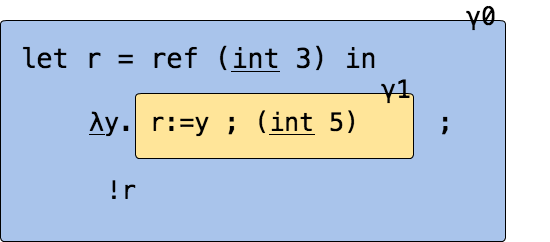
\includegraphics[clip,width=5cm]{./img/sudo_ref.png}
  危険な例
\end{center}
ここで,$r$は,整数のコードを格納する参照(破壊的セル)であり,$r:=y$と
$!r$はそれぞれ,$r$への代入と$r$の中身の読み出しを表す.
上記のプログラムは,コードレベルのラムダ抽象($y$に対するラムダ抽象)で
生成されるコードレベル変数を$u$とするとき,$\code{u}$を$r$に格納し,
$u$のスコープ(黄色で示したもの)が終わったあとに取り出しているため,
計算結果は,自由変数をもつコード$\code{u}$となり,危険である.

上記のようなプログラムを型エラーとするため,須藤らは,コードレベル変数の
スコープごとに環境識別子を割り当てた.
上記では外側のスコープ(青)が$\gamma_0$,
内側のスコープ(黄)が$\gamma_1$という環境識別子で表現される.
$\gamma_0$で有効なコードレベル変数はなく,
$\gamma_1$で有効なコードレベル変数は$y$(に対応して生成される変数)である.
$\gamma_0$のスコープは$\gamma_1$のスコープを含む.言い換えれば,
$\gamma_1$で使える変数の方が$\gamma_0$で使える変数の方が(同じか)多い.
このことを$\gamma_1 \ord \gamma_0$ と表すことにする.
$r$は $\codeT{\intT}{\gamma_0} \mbox{\texttt{ref}}$型を持つ.
$y$は $\gamma_1$で使える変数であるが,$\gamma_0$では使えないため,
$r$に$y$を代入することはできず,$r:=y$のところで型エラーとなる.

コードレベルの変数スコープと,型によるスコープの表現をあらわしたのが,以下の図である.
forやletなどコードレベルの束縛子があるたびに,新しいスコープが開かれ,
使える変数が増えていくことが分かるだろう.
\begin{center}
  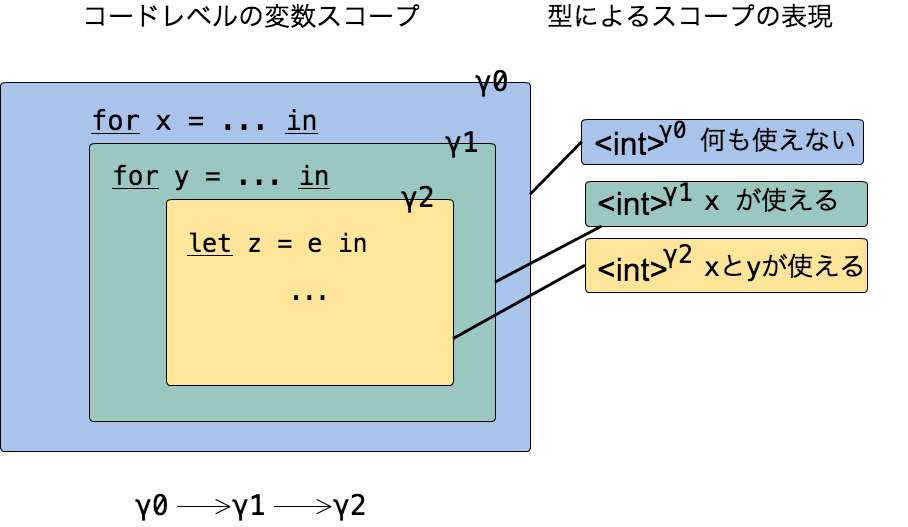
\includegraphics[clip,height=4cm]{./img/ec_for.png}
\end{center}

コードレベルの変数の型に,(精密化した)環境識別子を付与することで,その
変数が使えるスコープがわかり,破壊的代入などの副作用があるプログラムにおいても
スコープや型の安全性を保つことができる.

なお,須藤らの対象としていた言語が持っていた計算エフェクトは,「局所的なスコープをもつ参照」
であり,現実のOCaml/MetaOCaml等とは異なるものであった.
同一の著者グループは,最近,精密化した環境識別子のアイディアを用いて,
グローバルな参照を持つ言語に対するある種の型安全性
が成立することを示している\cite{Aplas2016}.

\section{本研究: 環境識別子の拡張}

本研究で扱う shift0/reset0によるコントロールエフェクトは,
須藤らによる精密化された環境識別子でも扱うことができない.本節では,そ
の問題点を明らかにし,その問題の解決の鍵となる join ($\cup$)の導入につ
いて述べる.

このため,前述の2重のforループ生成において,その中間にlet挿入をするプログラムに
ついて考察する.その概形は下記の1つ目の図である.
\begin{center}
  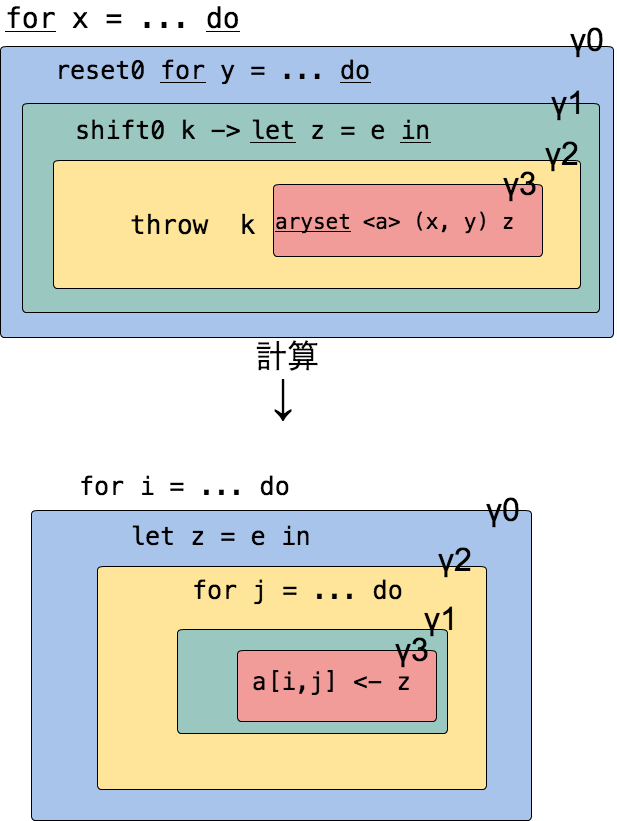
\includegraphics[clip,height=8cm]{./img/ecex_for_non_gamma.png}
\end{center}
上の方の図で,使えるコードレベル変数が異なる場所ごとに,
$\gamma_0,\gamma_1,\gamma_2,\gamma_3$と名付けた.
須藤らの体系通りであれば,これらの環境識別子の間の順序は,スコープの包
含関係通りであるので,
\begin{center}
  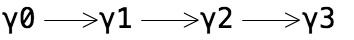
\includegraphics[clip,width=4cm]{./img/gamma_normal.png}
\end{center}
という順序がつくはずである.
しかし,計算を進めて得られたコードを見ると(上記の下の図はコードの中身を示している),
$\gamma_1$(緑色)と$\gamma_2$(黄色)の位置関係が入れ代わっている.
結果のコードの型が整合する(束縛変数が自由になることはない等)ために
は,$\gamma_2$において$\gamma_1$で使える変数を使ってはいけないことがわかる.
一方で,赤字で示された$\gamma_3$においては,$\gamma_1$の変数も
$\gamma_2$の変数も使って構わない.
これらを考慮すると,環境識別子の間の順序は以下の図となる.
\begin{center}
  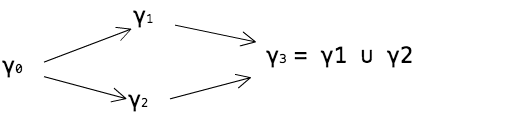
\includegraphics[clip,width=7cm]{./img/gamma.png}
\end{center}
ここでのポイントは,$\gamma_0$ から,2つの異なる(包含関係のな
い)$\gamma_1$と$\gamma_2$に別れたあと,再び$\gamma_3$で合流することで
ある.須藤らの体系では,環境識別子のなす半順序集合全体は木の形であったが,
本研究の体系では,このように1度別れたものが合流することがある.
なお,$\gamma_3$で使える変数の集合は$\gamma_1$と$\gamma_2$で使える変数の和集
合と一致するので$\gamma_3 = \gamma_1 \cup \gamma_2$とおくことができる.
このように,環境識別子の世界に Join ($\cup$)を導入することによ
り,コントロールオペレータによる文脈の移動に対応できることになった.

\section{本研究: 型システムの構築}

本研究の基本アイディアは前項で述べたようなシンプルなものであるが,
言語体系と型システムの構築にあたってはいくつかの困難があった.
ここでは,そのうち,コントロールオペレータが切りとった継続に関する多相性について述べる.

前節の例では,shift0 が切り取る文脈(継続)は,
穴が$\gamma_1$のスコープにあり(その型は $\codeT{t_1}{\gamma_1}$の型),
文脈全体が$\gamma_0$のスコープのにある(その型は
$\codeT{t_0}{\gamma_0}$の形)となっている.
これをthrowにおいて使うときは,$\gamma_3$スコープのものを$\gamma_2$ス
コープに変換している.すなわち,$k$は $\codeT{t_1}{\gamma_3}$型
から$\codeT{t_0}{\gamma_2}$型への関数であるように振る舞う.

この2つのギャップを埋めるのは,継続(評価文脈)のある種の多相性である.
このケースでは,
\[\codeT{t_1}{\gamma_1} \to \codeT{t_0}{\gamma_0} \]
という型で定義された継続変数$k$が,任意の$\gamma_2 \ord \gamma_0$ に対して,
\[\codeT{t_1}{\gamma_1 \cup \gamma_2} \to \codeT{t_0}{\gamma_0 \cup \gamma_2} \]
という型を持つことが言えれば良いことがわかる.($\gamma_3 = \gamma_1
\cup \gamma_2$あること,また,$\gamma_2 \ord \gamma_0$ ならば
$\gamma_0 \cup \gamma_2 = \gamma_2$であることに注意されたい.)

このような多相性(サブタイプのもとでの多相性)は,継続の研究ではいくつか
知られており,今回のケースでも成立すると考えられる\footnote{この型付
  けが問題ないことは直感的には明らかであるが,
  意味論の上で,このような型付け規則が「正しい」ことの証明は,将来課題である.}.

本研究では,将来的に型推論アルゴリズムを構築することを考慮して,
環境識別子に関する一般的な多相性を導入することを避け,
継続変数について特別な型を与え,その変数をthrowで使うときに,
多相性を利用できるようにするという方策をとった.これにより型システムを
複雑化させることなく,コントロールオペレータの導入ができ,簡潔な型保存
性の証明につながった.

最終的に得られた throw の型付け規則は以下のものであり,
継続変数$k$ には,特別な関数型$\Rightarrow$を与えていること(通常の関数
型は$\rightarrow$で表現している),また,
$\gamma_1$から$\gamma_0$への変換子として得られた$k$を,
$\gamma_1\cup \gamma_2$から$\gamma_2 = \gamma_0 \cup \gamma_2$への
変換子として利用していることがわかる.
\[
  \infer
  {\Gamma,~k:\contT{\codeT{t_1}{\gamma_1}}{\codeT{t_0}{\gamma_0}}{\sigma}
    \vdash \throw{k}{v} : \codeT{t_0}{\gamma_2} ; \sigma}
  {\Gamma
    \vdash v : \codeT{t_1}{\gamma_1 \cup \gamma_2} ; \sigma
    & \Gamma \models \gamma_2 \ord \gamma_0
  }
\]

なお,継続が作用する型(上記の$\codeT{t_1}{\gamma_1}$など)は,本研究で
はコード型に限定した.その理由は,須藤らの体系の方式で,参照(ref)が関
数型を持つことを許すとコードレベル変数が束縛域を脱出してしまい,
本研究のコントロールオペレータを持つ体系でも同様の事態が生じると予想さ
れたからである.
なお,コード型のみを扱うことのできるコントロールオペレータであっても,
多段階let挿入の表現のためには十分である.

%%% Local Variables:
%%% mode: japanese-latex
%%% TeX-master: "master_oishi"
%%% End:

\chapter{対象言語: 構文と意味論}

本研究における対象言語は,ラムダ計算にコード生成機能とコントロールオペ
レータshift0/reset0を追加したものに型システムを導入したものである.

本稿では,最小限の言語のみについて考えるため,コード生成機能の
「ステージ(段階)」は,コード生成段階(レベル0,現在ステージ)と
生成されたコードの実行段階(レベル1,将来ステージ)の2ステージのみを考える.

前述したように,本研究の言語では,
コードコンビネータ(Code Combinator)方式を使い,
コードコンビネータは,
$\cPlus$ や $\cIf$のように下線を引いて表す.

\section{構文の定義}

対象言語の構文を定義する.

変数は,レベル0変数($x$), レベル1変数($u$),
(レベル0の)継続変数($k$)の3種類がある.
レベル0項($e^0$),レベル1項($e^1$)およびレベル0の値($v$)を下の通り定義する.

\begin{align*}
  c & ::= i \mid b \mid \cint
      \mid \cat \mid + \mid \cPlus \mid \cIf \\
  v & ::= x \mid c \mid \fun{x}{e^0} \mid \code{e^1} \\
  e^0 & ::=  v  \mid e^0~ e^0 \mid \ift{e^0}{e^0}{e^0} \\
    & \mid \cfun{x}{e^0}
      \mid \ccfun{u}{e^0} \\
    & \mid \resetz{e^0}
      \mid \shiftz{k}{e^0}
      \mid \throw{k}{v} \\
  e^1 & ::=  u \mid c \mid \fun{u}{e^1} \mid e^1~ e^1
        \mid \ift{e^1}{e^1}{e^1} \\
\end{align*}
ここで$i$は整数の定数,$b$は真理値定数である.

定数のうち,下線がついているものはコードコンビネータである.
変数は,ラムダ抽象(下線なし,下線つき,二重下線つき)および shift0 により束縛され,
$\alpha$同値な項は同一視する.
$\letin{x}{e_1}{e_2}$および$\clet{x}{e_1}{e_2}$は,
それぞれ,$(\fun{x}{e_2})e_1$
$(\cfun{x}{e_2})\cat e_1$の省略形である.
前述の例でのべた$\cFor$は,
コード構築定数とコードレベル適用$\cap$を用いて導入することとし,
(この導入にあたっての型システムの拡張は容易なので)ここでは省略する.

\section{操作的意味論}

対象言語は,値呼びで left-to-rightの操作的意味論を持つ.
ここでは評価文脈に基づく定義を与える.

評価文脈を以下のように定義する.
\begin{align*}
  E & ::= [~] \mid E~ e^0 \mid v~ E \\
    & \mid \ift{E}{e^0}{e^0} \mid \Resetz~ E \mid \ccfun{u}{E}
\end{align*}
コード生成言語で特徴的なことは,
コードレベルのラムダ抽象の内部で評価が進行する点である.実際,
上記の定義には,$\ccfun{u}{E}$が含まれている.
たとえば,$\ccfun{u}{u \cPlus [~]}$ は評価文脈である.

この評価文脈$E$と次に述べる計算規則$r \to l$ により,
評価関係$e \lto e'$ を次のように定義する.
\[
  \infer{E[r] \lto E[l]}{r \to l}
\]

計算規則は以下の通り定義する.
\begin{align*}
  (\fun{x}{e})~v &\to e\{ x := v \} \\
  \ift{true}{e_1}{e_2} &\to e_1 \\
  \ift{else}{e_1}{e_2} &\to e_2 \\
  \cfun{x}{e} &\to \ccfun{u}{(e\{ x := \code{u} \})} \\
  \ccfun{u}{\code{e}} &\to \code{\fun{u}{e}} \\
  \Resetz~ v &\to v \\
  \Resetz (E[\Shiftz~ k \to e]) &\to e \ksubst{k}{E}
\end{align*}
ただし,4行目の$u$はフレッシュなコードレベル変数とし,
最後の行の$E$は穴の周りに{\Resetz}を含まない評価文脈とする.
また,この行の右辺のトップレベルに{\Resetz}がない点が,
shift/reset の振舞いとの違いである.すなわち,shift0 を1回計算すると,
reset0 が1つはずれるため,shift0 をN個入れ子にすることにより,
N個分外側のreset0 までアクセスすることができ,多段階let挿入を実現でき
るようになる.

上記における継続変数に対する代入$e\ksubst{k}{E}$は次の通り定義する.
\begin{align*}
  (\throw{k}{v})\ksubst{k}{E} &\equiv \Resetz (E[v]) \\
  (\throw{k'}{v})\ksubst{k}{E} &\equiv \throw{k'}{(v\ksubst{k}{E})}
  \\
                              & \text{ただし}~k \not= k'
\end{align*}
上記以外の$e$に対する代入の定義は透過的であるとする.
上記の定義の1行目で\Resetz を挿入しているのは{\Shiftz}の意味論に対応し
ており,これを挿入しない場合は別のコントロールオペレータ(Felleisenの
control/promptに類似した control0/prompt0)の振舞いとなる.

コードコンビネータ定数の振舞い(ラムダ計算における$\delta$規則に相当)は
以下のように定義する.

\begin{align*}
  \cint~ n &\to \code{n} \\
  \code{e_1}~ \cat~ \code{e_2} &\to \code{e_1~ e_2} \\
  \code{e_1}~ \cPlus~ \code{e_2} &\to \code{e_1 + e_2} \\
  \cif{e_1}{e_2}{e_3} &\to \code{\ift{e_1}{e_2}{e_3}}
\end{align*}

% 計算の例を以下に示す.
% \begin{align*}
%   e_1 & = \Resetz ~~\cLet~x_1=\csp{3}~\cIn \\
%   & \phantom{=}~~ \Resetz ~~\cLet~x_2=\csp{5}~\cIn \\
%   & \phantom{=}~~ \Shiftz~k~\to~\cLet~y=t~\cIn \\
%   & \phantom{=}~~ \Throw~ k~ (x_1~\cPlus~x_2~\cPlus~y) \\
% \end{align*}
%
% \begin{align*}
%   [ e_1 ] &\lto [ \Resetz (\cLet~x_1=\csp{3}~\cIn \\
%   &\Resetz~ \cLet~x_2=\csp{5}~\cIn \\
%   &[ \Shiftz~ k~ \to~ \cLet~ y=t~ \cIn \\
%   &[ \Throw~ k~(x_1~\cPlus~x_2~\cPlus~y) ] ] ) ] \\
%   &\lto [ \cLet~ y=t~ \cIn \\
%   &[ \cfun{x}{\Resetz~ (\cLet~x_1=\csp{3}~ \cIn~ \Resetz~ (\cLet~ x_2=\csp{5}~ \cIn [x]))} (x_1~\cPlus~x_2~\cPlus~y) ]] \\
%   &\lto [ \cfun{y}{(\cfun{x}{\Resetz~ (\cLet~x_1=\csp{3}~ \cIn~ \Resetz~ (\cLet~ x_2=\csp{5}~ \cIn [x]))} (x_1~\cPlus~x_2~\cPlus~y))}~ \cat~ t ] \\
%   &\lto [[\cfun{y}{(\cfun{x}{\Resetz~ (\cLet~x_1=\csp{3}~ \cIn~ \Resetz~ (\cLet~ x_2=\csp{5}~ \cIn [x]))} (x_1~\cPlus~x_2~\cPlus~y))}]~ \cat~ t] \\
%   &\lto [[\ccfun{y_1}{(\cfun{x}{\Resetz~ (\cLet~x_1=\csp{3}~ \cIn~ \Resetz~ (\cLet~ x_2=\csp{5}~ \cIn [x]))} (x_1~\cPlus~x_2~\cPlus~ \code{y_1}))}]~ \cat~ t] \\
%   &\lto
% \end{align*}

%%% Local Variables:
%%% mode: japanese-latex
%%% TeX-master: "master_oishi"
%%% End:

\chapter{型システム}

本研究での型システムについて述べる.

基本型$b$,環境識別子(Environment Classifier)$\gamma$を以下の通り定義する.
\begin{align*}
  b & ::= \intT \mid \boolT \\
  \gamma & ::= \gamma_x \mid \gamma \cup \gamma
\end{align*}
$\gamma$の定義における$\gamma_x$は環境識別子の変数を表す.
すなわち,環境識別子は,変数であるかそれらを$\cup$で結合した形である.
以下では,メタ変数と変数を区別せず$\gamma_x$を$\gamma$と表記する.
ここで環境識別子として$\cup$を導入した理由は後述する.

$L ::= \empty \mid \gamma$ は現在ステージと将来ステージをまとめ
て表す記号である.たとえば,$\Gamma \vdash^L
e:t~;~\sigma$は,$L=\empty$のとき現在ステージの判断で,
$L=\gamma$のとき将来ステージの判断となる.

レベル0の型$t^0$,レベル1の型$t^1$,(レベル0の)型の有限列$\sigma$,
(レベル0の)継続の型$\kappa$を次の通り定義する.
\begin{align*}
  t^0 & ::= b \mid \funT{t^0}{t^0}{\sigma} \mid \codeT{t^1}{\gamma} \\
  t^1 & ::= b \mid t^1 \to t^1 \\
  \sigma & ::= \epsilon \mid \sigma,t^0 \\
  \kappa^0 & ::= \contT{\codeT{t^1}{\gamma}}{\codeT{t^1}{\gamma}}{\sigma}
\end{align*}

レベル0の関数型$\funT{t^0}{t^0}{\sigma}$は,
エフェクトをあらわす列$\sigma$を伴っている.これは,その関数型をもつ項
を引数に適用したときに生じる計算エフェクトであり,具体的には,
\Shiftz の answer type の列である.前述したようにshift0 は多段
階の reset0 にアクセスできるため,$n$個先のreset0 の answer typeまで記
憶するため,このように型の列$\sigma$で表現している.
ただし,本研究の範囲では,answer type modification に対応する必要はな
いので,エフェクトはシンプルに型の列($n$個先の reset0 のanswer type を
$n=1,\cdots,k$に対して並べた列)で表現している.
この型システムの詳細は,Materzokら\cite{Materzok2011}の研究を参照されたい.

本稿の範囲では,コントロールオペレータは現在ステージのみにあらわれ,生
成されるコードの中にはあらわないため,レベル1の関数型は,エフェクトを
表す列を持たない.
また,本項では,shift0/reset0 はコードを操作する目的にのみ使うため,継
続の型は,コードからコードへの関数の形をしている.
ここでは,後の定義を簡略化するため,継続を,通常の関数とは区別しており,
そのため,継続の型も通常の関数の型とは区別して二重の横線で表現している.

型判断は,以下の2つの形である.
\begin{align*}
  \Gamma \vdash^{L} e : t ;~\sigma \\
  \Gamma \models \gamma \ord \gamma
\end{align*}
ここで,型文脈$\Gamma$は次のように定義される.
\begin{align*}
  \Gamma ::= \emptyset
  \mid \Gamma, (\gamma \ord \gamma)
  \mid \Gamma, (x : t)
  \mid \Gamma, (u : t)^{\gamma}
\end{align*}

型判断の導出規則を与える.まず,$\Gamma \models \gamma \ord \gamma$の
形に対する規則である.

\[
  \infer
  {\Gamma \models \gamma_1 \ord \gamma_1}
  {}
  \quad
  \infer
  {\Gamma, \gamma_1 \ord \gamma_2 \models \gamma_1 \ord \gamma_2}
  {}
\]

\[
  \infer
  {\Gamma \models \gamma_1 \ord \gamma_3}
  {\Gamma \models \gamma_1 \ord \gamma_2 & \Gamma \models \gamma_2 \ord \gamma_3}
\]

\[
  \infer
  {\Gamma \models \gamma_1 \cup \gamma_2 \ord \gamma_1}
  {}
  \quad
  \infer
  {\Gamma \models \gamma_1 \cup \gamma_2 \ord \gamma_2}
  {}
\]

\[
  \infer
  {\Gamma \models \gamma_3 \ord \gamma_1 \cup \gamma_2}
  {\Gamma \models \gamma_3 \ord \gamma_1
    &\Gamma \models \gamma_3 \ord \gamma_2}
\]



次に,$\Gamma \vdash^{L} e : t ;~\sigma$ の形に対する導出規則を与える.
まずは,レベル0における単純な規則である.

\[
  \infer
  {\Gamma, x : t \vdash x : t ~;~ \sigma}
  {}
  \quad
  \infer
  {\Gamma, (u : t)^\gamma \vdash^\gamma u : t ~;~ \sigma}
  {}
\]

\[
  \infer
  {\Gamma \vdash^{L} c : t^c ~;~\sigma}
  {}
\]

\[
  \infer
  {\Gamma \vdash^{L} e_1~ e_2 : t_1 ; \sigma}
  {\Gamma \vdash^{L} e_1 : t_2 \to t_1 ; \sigma
    & \Gamma \vdash^{L} e_2 : t_2  ; \sigma
  }
\]

\[
  \infer
  {\Gamma \vdash \fun{x}{e} : \funT{t_1}{t_2}{\sigma} ~;~\sigma'}
  {\Gamma,~x : t_1 \vdash e : t_2 ~;~ \sigma}
  \quad
  \infer
  {\Gamma \vdash^\gamma \fun{x}{e} : \funT{t_1}{t_2}{} ~;~\sigma'}
  {\Gamma,~(u : t_1)^\gamma \vdash^\gamma e : t_2 ~;~ \sigma}
\]

\[
  \infer
  {\Gamma \vdash^{L} \ift{e_1}{e_2}{e_3} : t ~;~ \sigma}
  {\Gamma \vdash^{L} e_1 : \boolT ;~ \sigma
    & \Gamma \vdash^{L} e_2 : t ; \sigma
    & \Gamma \vdash^{L} e_3 : t ; \sigma}
\]

次にコードレベル変数に関するラムダ抽象の規則である.

\[
  \infer[(\gamma_1~\text{is eigen var})]
  {\Gamma \vdash \cfun{x}{e} : \codeT{t_1\to t_2}{\gamma} ~;~ \sigma}
  {\Gamma,~\gamma_1 \ord \gamma,~x:\codeT{t_1}{\gamma_1} \vdash e
    : \codeT{t_2}{\gamma_1}; \sigma}
\]

\[
  \infer
  {\Gamma \vdash \ccfun{u^1}{e} : \codeT{t_1 \to t_2}{\gamma} ; \sigma}
  {\Gamma, \gamma_1 \ord \gamma, x : (u : t_1)^{\gamma_1} \vdash e : \codeT{t_2}{\gamma_1} ; \sigma}
\]

コントロールオペレータに対する型導出規則である.

\[
  \infer{\Gamma \vdash \resetz{e} : \codeT{t}{\gamma} ~;~ \sigma}
  {\Gamma \vdash e : \codeT{t}{\gamma} ~;~ \codeT{t}{\gamma}, \sigma}
\]

\[
  \infer{\Gamma \vdash \shiftz{k}{e} : \codeT{t_1}{\gamma_1} ~;~ \codeT{t_0}{\gamma_0},\sigma}
  {\Gamma,~k:\contT{\codeT{t_1}{\gamma_1}}{\codeT{t_0}{\gamma_0}}{\sigma}
    \vdash e : \codeT{t_0}{\gamma_0} ; \sigma
    & \Gamma \models \gamma_1 \ord \gamma_0
  }
\]

\[
  \infer
  {\Gamma,~k:\contT{\codeT{t_1}{\gamma_1}}{\codeT{t_0}{\gamma_0}}{\sigma}
    \vdash \throw{k}{v} : \codeT{t_0}{\gamma_2} ; \sigma}
  {\Gamma
    \vdash v : \codeT{t_1}{\gamma_1 \cup \gamma_2} ; \sigma
    & \Gamma \models \gamma_2 \ord \gamma_0
  }
\]

コード生成に関する補助的な規則として,Subsumptionに相当する規則等がある.
\[
  \infer
  {\Gamma \vdash e : \codeT{t}{\gamma_2} ; \sigma}
  {\Gamma \vdash e : \codeT{t}{\gamma_1} ; \sigma
    & \Gamma \models \gamma_2 \ord \gamma_1
  }
\]

\[
  \infer
  {\Gamma \vdash^{\gamma_2} e : t ~;~ \sigma}
  {\Gamma \vdash^{\gamma_1} e : t ~;~ \sigma
    & \Gamma \models \gamma_2 \ord \gamma_1
  }
\]


\[
  \infer
  {\Gamma \vdash \code{e} : \codeT{t^1}{\gamma} ; \sigma}
  {\Gamma \vdash^{\gamma} e : t^1 ; \sigma}
\]


\section{型付け例}

上記の型システムのもとで,いくつかの項の型付けについて述べる.

\begin{align*}
  e_1 & = \Resetz ~~\cLet~x_1=\csp{3}~\cIn \\
      & \phantom{=}~~ \Resetz ~~\cLet~x_2=\csp{5}~\cIn \\
      & \phantom{=}~~ \Shiftz~k~\to~\cLet~y=t~\cIn \\
      & \phantom{=}~~ \Throw~k~(x_1~\cPlus~x_2~\cPlus~y)
\end{align*}

この式$e_1$に対して,もし,$t=\csp{7}$ あるいは $t=x_1$であれば,
$e_1$ は型付け可能である.
一方,$t=x_2$ であれば,$e_1$ は型付けできない.

\begin{align*}
  e_2 & = \Resetz ~~\cLet~x_1=\csp{3}~\cIn \\
      & \phantom{=}~~ \Resetz ~~\cLet~x_2=\csp{5}~\cIn \\
      & \phantom{=}~~ \Shiftz~k_2~\to~ \Shiftz~k_1~\to~ \cLet~y=t~\cIn \\
      & \phantom{=}~~ \Throw~k_1~(\Throw~k_2~(x_1~\cPlus~x_2~\cPlus~y))
\end{align*}

この式$e_2$に対して,もし$t=\csp{7}$であれば$e_1$は型付け可能である.
一方,$t=x_2$ あるいは $t=x_1$であれば,$e_1$は型付けできない.

このように,(少なくとも)上記の例については安全な式と危険な式を正しく峻
別できていることがわかった.

\section{型安全性について}

本研究の型システムに対する型保存(Subject Reduction)定理について述べる.
型保存定理は,(証明できれば)
進行(Progress)定理とあわせて型システムの健全性を導く定理である.

\begin{quote}
  (型保存性)
  $\vdash e:t~;~\sigma$ かつ $e \lto e'$ であれば,$\vdash e':t~;~\sigma$
  である.
\end{quote}

この定理は reset0-shift0の計算規則が多相性を持たない場合には容易に証明
できるが,多相性については精密な扱いが必要であり,
現段階では,型保存定理の証明は進行中である.

% \begin{lemm}[不要な仮定の除去]
%   $\Gamma_1,\gamma_2 \ord \gamma_1 \vdash e : t_1 ~;~\sigma$
%   かつ,$\gamma_2$が $\Gamma_1, e, t_1, \sigma$に出現しないなら,
%   $\Gamma_1 \vdash e : t_1 ~;~\sigma$ である.
% \end{lemm}
%
% \begin{lemm}[値に関する性質]
%   $\Gamma_1 \vdash v : t_1 ~;~\sigma$
%   ならば,
%   $\Gamma_1 \vdash v : t_1 ~;~\sigma'$
%   である.
% \end{lemm}
%
% \begin{lemm}[代入]
%   $\Gamma_1, \Gamma_2, x : t_1 \vdash e : t_2 ~;~\sigma$
%   かつ
%   $\Gamma_1 \vdash v : t_1 ~;~\sigma$
%   ならば,
%   $\Gamma_1, \Gamma_2 \vdash e\{x := v\} : t_2~;~\sigma$
% \end{lemm}
%
% これらをもとに型保存定理を証明する.
% 本研究の対象言語は,コントロールオペレータが操作する対象となる式の型を
% コード型に限定するなど,注意深く設計しているので,ほとんどのケースの証
% 明はスムーズであるが,reset0-shift0 に関する計算規則(shift0 が評価文脈
% を捕捉して継続変数$k$に渡す規則)とthrowに関する計算規則では,
% サブタイプ多相性に相当する性質を使っているので,以下の技術的な補題が必
% 要である.
%
% \begin{lemm}[識別子に関する多相性]
%   穴の周りにreset0を含まない評価文脈$E$,変数$x$,
%   そして$\Gamma = (u_1:t_1)^{\gamma_1}, \cdots, (u_n:t_n)^{\gamma_n}$
%   かつ$i=1,\cdots,n$に対して$\Gamma \models \gamma_0 \ord \gamma_i$であるとする.
%   このとき,
%   $\Gamma, x:\codeT{t_0}{\gamma'} \vdash E[x] : \codeT{t_1}{\gamma_0} ~;~\sigma$
%   であれば,フレッシュな$\gamma$に対して,
%   $\Gamma, x:\codeT{t_0}{\gamma'\cup \gamma} \vdash
%   E[x] : \codeT{t_1}{\gamma_0 \cup \gamma} ~;~\sigma$
%   である.
% \end{lemm}
%
% この補題は,評価文脈$E$に対して,穴の型が$\codeT{t_0}{\gamma'}$で
% 評価文脈全体の型が$\codeT{t_1}{\gamma_0}$であれば,
% それぞれの環境識別子に$\gamma_2$を加えて,
% $\codeT{t_0}{\gamma'\cup \gamma}$型から,
% $\codeT{t_1}{\gamma_0\cup \gamma}$型への評価文脈として使ってもよい,
% ということを主張している.ここで $\gamma \ord \gamma_0$ なので,
% $\gamma$と$\gamma_0 \cup \gamma$は$\ord$の意味で等しくなり,
% $\codeT{t_1}{\gamma_0\cup\gamma}$型を持つ項は,
% $\codeT{t_1}{\gamma}$型も持つことがわかる.
% この定理により,shift0が捕捉した継続を(環境識別子について)多相的に使う
% ことが可能となり,reset0-shift0 の計算規則が正当化される.
%
% 上記の補題を証明すれば,型保存定理の証明の残りのケースは比較的容易であ
% る.なお,この補題を使うケースにおいて,定理の言明にあらわれる項$e$が
% 閉じた項であること(環境識別子に関する
%
%
% 進行定理については
% 精密な定式化が必要(reset0がない式でshift0を実行した時など)が必要なので,

% \section{進行}
% \begin{theo}[進行]
%   $\vdash e:t$ が導出可能であれば,$e$ は 値 $v$ である.または,$e \lto e'$ であるような 項 $e'$ が存在する
% \end{theo}
%
% \paragraph{証明}
% $\vdash e:t$ の導出に関する帰納法による.\\
% Const, Abs, Code 規則の場合 $e$ は値である.\\
% Var 規則の場合 $\vdash e:t$ は導出可能でない.\\
% Throw 規則の場合 $\vdash e:t$ は導出可能でない.\\
% Reset0 規則の場合 $e = \Resetz~ e_1$ とする.
% 帰納法の仮定より評価文脈における $\Resetz E$ より簡約が進み,\\
% $e_1$ が値のとき,$e \lto v$ となるような $v$ が存在する.\\
% $e_1$ が値でないとき,

%%% Local Variables:
%%% mode: japanese-latex
%%% TeX-master: "master_oishi"
%%% End:

\chapter{型安全性の証明}

\section{型保存}

\section{進行}

%%% Local Variables:
%%% mode: japanese-latex
%%% TeX-master: "master_oishi"
%%% End:
\chapter{まとめと今後の課題}
本研究では,効率的コード生成に有用な技法であるlet挿入を,型安全に実現す
るための言語と型システムについて述べた.
局所的な代入可能変数を持つ体系に対する須藤らの研究\cite{Sudo2014}などに基づき,
多段階のforループを飛び越えたlet挿入を実現するために,shift0/reset0 を持つコード生成体系を設計した.
須藤らの研究で精密化された環境識別子(Environment Classifier)に join ($\cup$) を導入することで,
計算の順序を変更するようなコントロールオペレータ(shift0/reset0)を扱えるようにし,
安全に多段階の let挿入を行えるように型システムを構築した.
このようなlet挿入が束縛子を越えるケースは,ループにおける不変式の括り出
しなどの有用な最適化を含むが,これまでの研究では一般的なlet挿入を安全
に実現した体系の提案はなく,我々の知る限り本研究がはじめてである.

今後の課題として,まずあげられるのは,進行(Progress)の性質および型推論
アルゴリズムの開発である.また,理論的には Kiselyovらのグローバルな参
照を持つ体系との融合が可能になれば,広い範囲のコード生成技法・最適化技法
をカバーできるため極めて有用である.
また,既存のMetaOCaml との比較においては,
2レベルのみのコード生成に限定している点や
run (生成したコードの実行)や cross-stage persistence (現在ス
テージの値をコードに埋め込む機能)などに対応していない点が欠点であり,
これらの拡張が可能であるかどうかの検討は非常に興味深い将来課題である.

%%% Local Variables:
%%% mode: japanese-latex
%%% TeX-master: "master_oishi"
%%% End:

\chapter{まとめと今後の課題}
本研究では,効率的コード生成に有用な技法であるlet挿入を,型安全に実現す
るための言語と型システムについて述べた.
局所的な代入可能変数を持つ体系に対する須藤らの研究\cite{Sudo2014}などに基づき,
多段階のforループを飛び越えたlet挿入を実現するために,shift0/reset0 を持つコード生成体系を設計した.
須藤らの研究で精密化された環境識別子(Environment Classifier)に join ($\cup$) を導入することで,
計算の順序を変更するようなコントロールオペレータ(shift0/reset0)を扱えるようにし,
安全に多段階の let挿入を行えるように型システムを構築した.
このようなlet挿入が束縛子を越えるケースは,ループにおける不変式の括り出
しなどの有用な最適化を含むが,これまでの研究では一般的なlet挿入を安全
に実現した体系の提案はなく,我々の知る限り本研究がはじめてである.

今後の課題として,まずあげられるのは,進行(Progress)の性質および型推論
アルゴリズムの開発である.また,理論的には Kiselyovらのグローバルな参
照を持つ体系との融合が可能になれば,広い範囲のコード生成技法・最適化技法
をカバーできるため極めて有用である.
また,既存のMetaOCaml との比較においては,
2レベルのみのコード生成に限定している点や
run (生成したコードの実行)や cross-stage persistence (現在ス
テージの値をコードに埋め込む機能)などに対応していない点が欠点であり,
これらの拡張が可能であるかどうかの検討は非常に興味深い将来課題である.

%%% Local Variables:
%%% mode: japanese-latex
%%% TeX-master: "master_oishi"
%%% End:


\chapter*{謝辞}
\addcontentsline{toc}{chapter}{\numberline{}謝辞}
ありがとうありがとう
\newpage

\addcontentsline{toc}{chapter}{\numberline{}参考文献}
\renewcommand{\bibname}{参考文献}
\bibliographystyle{junsrt}
\bibliography {bibfile}

\end{document}

%%% Local Variables:
%%% mode: japanese-latex
%%% TeX-master: t
%%% End:
